\begin{center}

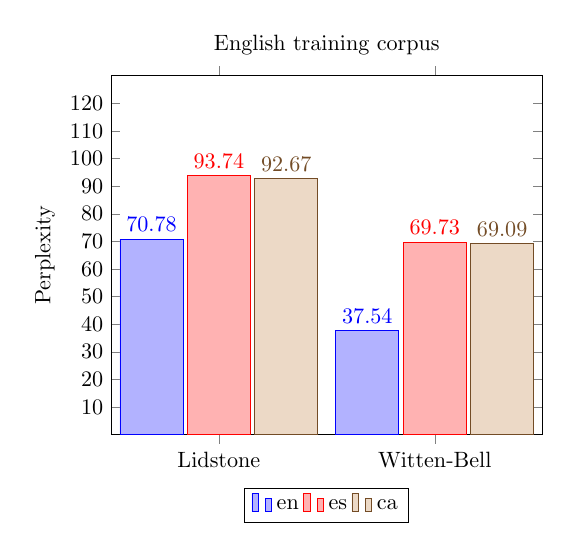
\begin{tikzpicture}[scale=.8]
\begin{axis}[
	title={English training corpus},
	ybar,
	enlarge x limits=0.5,
	legend style={at={(0.5,-0.15)}, anchor=north,legend columns=-1},
	ylabel={Perplexity},
	symbolic x coords={Lidstone,Witten-Bell},
	xtick=data,
	ymin=0, ymax=130,
	ytick={10,20,30,40,50,60,70,80,90,100,110,120},
	bar width=1cm,
	nodes near coords,
]
\addplot coordinates {(Lidstone,70.7838359216829787) (Witten-Bell,37.5384609732930841)};
\addplot coordinates {(Lidstone,93.7409203556402417) (Witten-Bell,69.7335551150016499)};
\addplot coordinates {(Lidstone,92.6689697631915124) (Witten-Bell,69.0850906203342134)};
\legend{en,es,ca}
\end{axis}
\end{tikzpicture}
\qquad
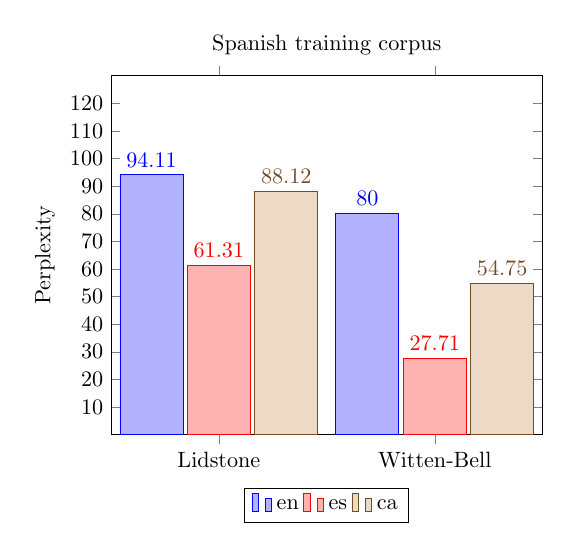
\begin{tikzpicture}[scale=.8]
\begin{axis}[
	title={Spanish training corpus},
	ybar,
	enlarge x limits=0.5,
	legend style={at={(0.5,-0.15)}, anchor=north,legend columns=-1},
	ylabel={Perplexity},
	symbolic x coords={Lidstone,Witten-Bell},
	xtick=data,
	ymin=0, ymax=130,
	ytick={10,20,30,40,50,60,70,80,90,100,110,120},
	bar width=1cm,
	nodes near coords,
]
\addplot coordinates {(Lidstone,94.1051565833287640) (Witten-Bell,79.9952132127366156)};
\addplot coordinates {(Lidstone,61.3100703532033791) (Witten-Bell,27.7121024323646807)};
\addplot coordinates {(Lidstone,88.1229201316707673) (Witten-Bell,54.7508602837030196)};
\legend{en,es,ca}
\end{axis}
\end{tikzpicture}

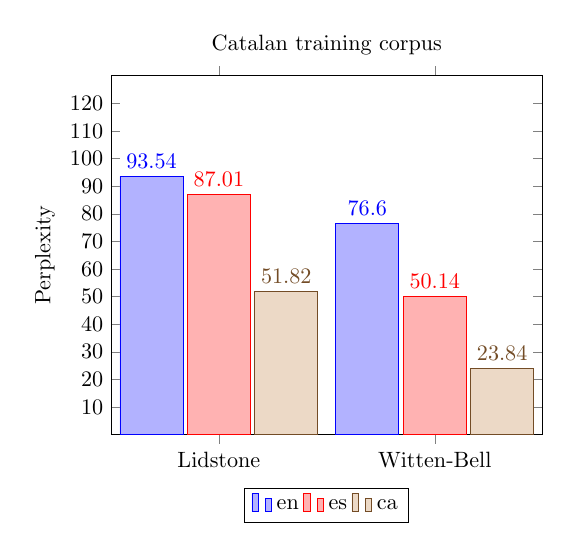
\begin{tikzpicture}[scale=.8]
\begin{axis}[
	title={Catalan training corpus},
	ybar,
	enlarge x limits=0.5,
	legend style={at={(0.5,-0.15)}, anchor=north,legend columns=-1},
	ylabel={Perplexity},
	symbolic x coords={Lidstone,Witten-Bell},
	xtick=data,
	ymin=0, ymax=130,
	ytick={10,20,30,40,50,60,70,80,90,100,110,120},
	bar width=1cm,
	nodes near coords,
]
\addplot coordinates {(Lidstone,93.5356597887484753) (Witten-Bell,76.5965039173272828)};
\addplot coordinates {(Lidstone,87.0130605277985296) (Witten-Bell,50.1368336506490166)};
\addplot coordinates {(Lidstone,51.8226074786520314) (Witten-Bell,23.8370767925576494)};
\legend{en,es,ca}
\end{axis}
\end{tikzpicture}

\end{center}